
\section{Analiza sistema}
Cilj ovog sistema jeste da olakša funkcionisanje jednog on-line restorana. To se postiže međusobnom komunikacijom korisnika, koordinatora kao i oso\-ba zaduženih za pripremu i distribuciju hrane. Na taj način realizuju se zahtevi korisnika u najkraćem vremenskom roku sa što boljim kvalitetom usluga.
%\subsection{Dijagram konteksta}

Na narednoj slici (Slika \ref{fig:slika1}) nalazi se dijagram konteksta koji grafički prikazuje osnovne aktere u sistemu i veze medju njima.


% \begin{center}
% 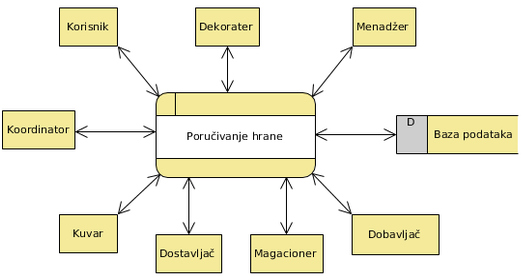
\includegraphics[width = 130mm]{slike/DC.jpg}
% \caption{Slika 1. Dijagram konteksta}
% \end{center}

\begin{figure}[ht]
    \leavevmode
    \begin{center}
    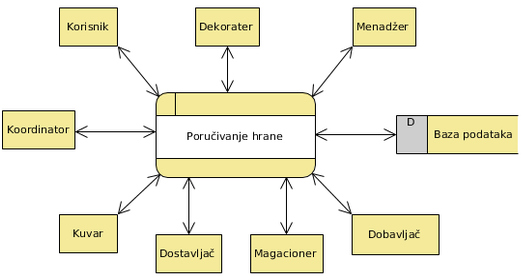
\includegraphics[height=0.3\textheight]{slike/DC.jpg}
    \end{center}
    \caption{Dijagram konteksta} % opis ce stajati ispod slike
    \label{fig:slika1}
\end{figure}


%Naime, korisniku je omogućeno da hranu naruči bilo putem telefona, bilo putem veb stranice.


%Ukoliko korisnik prvi put pristupa veb stranici radi naručivanja, neophodno je da se registruje sa ličnim podacima (ime, prezime, adresa, korisničko ime, lozinka...) dok svaki sledeći pristup stranici omogućen je običnom prijavom. Pored uobičajenih porudžbina, postoji i mogućnost aranžiranja i isporuke keteringa za različite tipove proslava.


%Sam restoran poseduje i sopstveni magacin za skladištenje svih potrebnih namirnica. Uz to, obezbeđeno je svo neophodno osoblje za koordinisanje ovakvog tipa restorana.


\subsection{Učesnici}
Glavna podela učesnika sistema je na:

\begin{itemize}
    \item Korisnik
    \begin{itemize}
        \item vrši porudžbine putem telefona ili veb stranice
        \item plaća dostavljaču utvrđeni iznos po prijemu paketa
    \end{itemize}
    \item Koordinator
    \begin{itemize}
        \item prihvata ili odbacuje narudžbinu od korisnika
        \item u slučaju prihvatanja obaveštava kuvara o detaljima porudžbine
        \item po prijemu paketa od kuvara ili dekoratera, prosleđuje ga dostavljaču uz napomenu o adresi korisnika
    \end{itemize}
    \item Kuvar
    \begin{itemize}
        \item priprema hranu zahtevanu od strane koordinatora
        \item u slučaju da je porudžbina tipa keteringa, pripremljenu hranu prosleđuje dekorateru
        \item po potrebi, obaveštava magacionera o nedovoljnim zalihama namirnica u kuhinji
    \end{itemize}
    \item Dostavljač
    \begin{itemize}
        \item preuzima iz kuhinje paket koji treba isporučiti, zajedno sa adresom isporuke i cenom
        \item isporučuje paket na datu adresu u najkraćem vremenskom roku
        \item obaveštava korisnika o ceni, vrši naplatu isporučenih dobara
        \item po potrebi, obaveštava menadžera o nedovoljnim zalihama goriva/potrebnim popravkama na vozilu za isporuke
    \end{itemize}
        \item Menadžer
    \begin{itemize}
        \item vodi računa o prilivu i odlivu novca restorana
        \item koordinira zaposlenima i njihovim nalozima
    \end{itemize}
    \newpage
    \item Magacioner
    \begin{itemize}
        \item vodi računa o količini zaliha namirnica u magacinu
        \item vrši prenos zahtevanih namirnica, od strane kuvara, u kuhinju
        \item vrši skladištenje pristiglih namirnica u magacin
        \item koordinira isporukama sa dobavljačem
    \end{itemize}
    \item Dekorater
    \begin{itemize}
        \item sarađuje sa kuvarom u aranžiranju keteringa
        \item završenu narudžbinu prosleđuje koordinatoru
    \end{itemize}
    \item Dobavljač
    \begin{itemize}
        \item vrši prijem dobara od strane distributera
        \item vrši isporuku dobara u magacin
    \end{itemize}
\end{itemize}


Sledeci DTP dijagram (Slika \ref{fig:slika2}) nivoa jedan predstavlja osnovne celine koje smo uočili. 
% \begin{center}
% 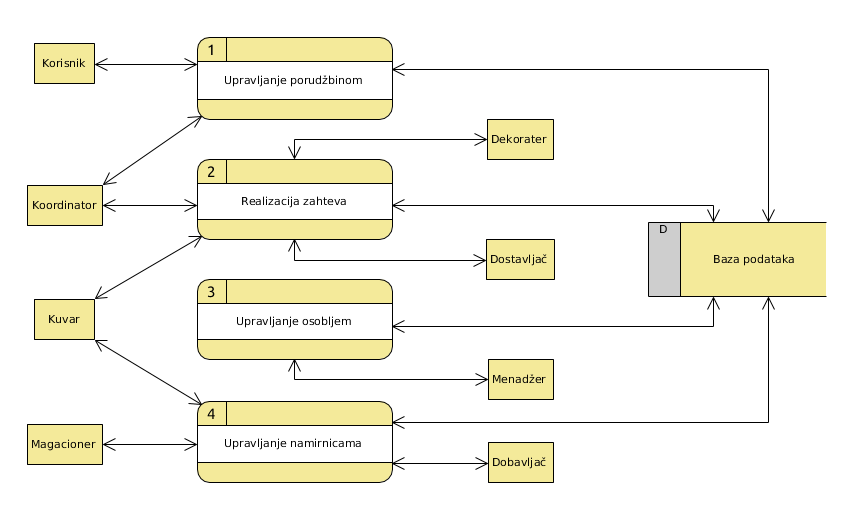
\includegraphics[width = 160mm]{slike/DTP.jpg}
% \caption{Slika 2. Dijagram toka podataka}
% \end{center}
\begin{figure}[ht]
    \leavevmode
    \begin{center}
    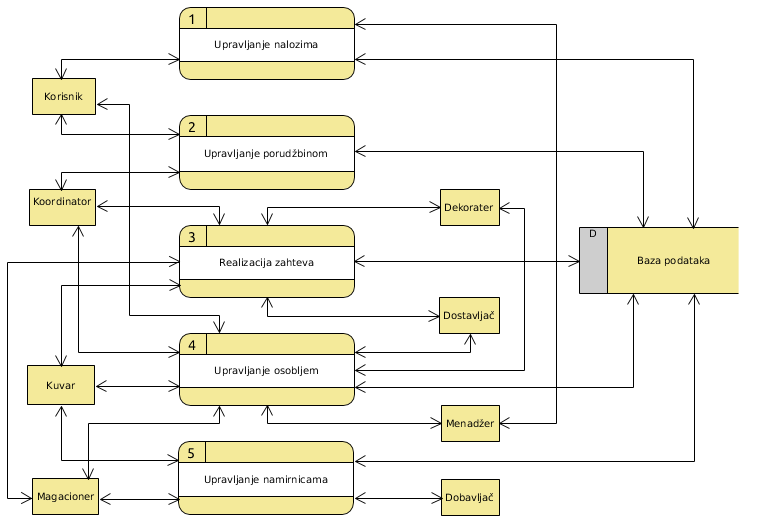
\includegraphics[height=0.55\textheight]{slike/DTP.png}
    \end{center}
    \caption{Dijagram toka podataka} % opis ce stajati ispod slike
    \label{fig:slika2}
\end{figure}
